\documentclass[11pt]{article}
\usepackage[letterpaper,margin=0.9in]{geometry}
\usepackage[T1]{fontenc}
\usepackage{lmodern,amsmath,amssymb,amsthm,mathtools,microtype,tikz,enumitem,booktabs,xurl}
\usepackage[colorlinks=true,linkcolor=black,citecolor=black,urlcolor=blue!45!black]{hyperref}
\setlength{\parindent}{0pt}
\setlength{\parskip}{5pt plus 1pt minus 1pt}
\setlength{\emergencystretch}{2em}
\setlist{nosep,leftmargin=1.5em,topsep=4pt}
\newtheorem{theorem}{Theorem}[section]
\newtheorem{lemma}[theorem]{Lemma}
\newtheorem{proposition}[theorem]{Proposition}
\newtheorem{corollary}[theorem]{Corollary}
\theoremstyle{definition}
\newtheorem{definition}[theorem]{Definition}
\newcommand{\Z}{\mathbb Z}
\newcommand{\R}{\mathbb R}
\newcommand{\intr}{\operatorname{int}}
\newcommand{\dist}{\operatorname{dist}}
\newcommand{\lcm}{\operatorname{lcm}}
\hypersetup{pdfauthor={Daniel Wang and Peyton Wang}}

\title{Illumination through long rectangular necks}
\author{Daniel Wang \and Peyton Wang}
\date{Working draft v0.1 --- November 8, 2026}
\begin{document}\maketitle
\begin{abstract}
Two fixed orthogonal polygonal chambers with smooth mouths of the same positive width are joined by a rectangular neck of length $L$. For each fixed opposing pair of interior marks, we prove illumination for every sufficiently large real $L$. The chamber dimensions and marks may be arbitrary real numbers. Directional minimality supplies two finite stable entrance beams; an exact arithmetic progression then matches the actual target. The threshold is locally uniform under nondegenerate perturbations. Separately, for a fixed tree of orthogonal chambers with parallel necks of commensurate widths, one supplied legal witness implies eventual illumination along nonnegative rational-affine neck-length growth. The network theorem assumes witness existence; the two-chamber theorem does not.
\end{abstract}

\section{Two fixed chambers}
All billiard paths in this paper have finitely many ordinary specular reflections and avoid every physical polygon corner. Fix $w>0$, and finite strictly simple orthogonal closed polygonal disks $C_-$ and $C_+$ in $x\le0$ and $x\ge0$, respectively. Each has $M=\{0\}\times[0,w]$ on its boundary, with all relative-interior points of $M$ smooth. Fix $S\in\intr C_-$ and $T\in\intr C_+$. Form
\[
 P_L=C_-\cup([0,L]\times[0,w])\cup(C_++(L,0)),\qquad T_L=T+(L,0).
\]
Assume these gluings have no additional contacts, so $P_L$ is a strictly simple disk. The former mouths are open passages.

\begin{theorem}\label{thm:neck}
There is a finite $L_0$, depending on the fixed chamber, mouth and mark data, such that $S$ illuminates $T_L$ in $P_L$ for every real $L>L_0$. The threshold is locally uniform when the wall patterns, positive mouths, strict simplicity and interior marks persist.
\end{theorem}

There is no rationality, area, wall-count or reflection-count assumption. The threshold is not claimed to depend only on the number of walls.

\begin{figure}[htbp]\centering
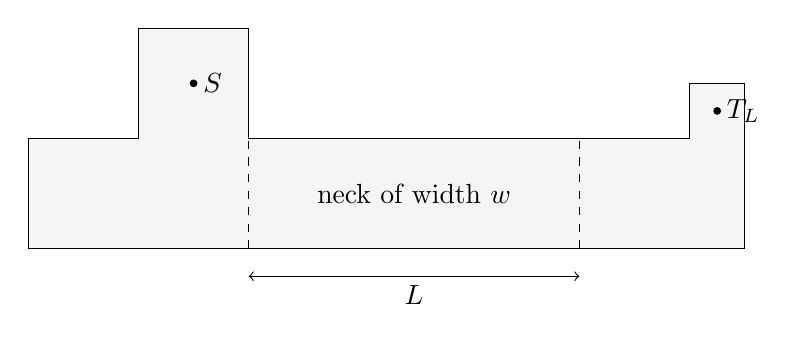
\begin{tikzpicture}[scale=.7]
\filldraw[fill=gray!8] (-4,0)--(0,0)--(6,0)--(9,0)--(9,3)--(8,3)--(8,2)--(6,2)--(0,2)--(0,4)--(-2,4)--(-2,2)--(-4,2)--cycle;
\draw[dashed] (0,0)--(0,2) (6,0)--(6,2);
\fill (-1,3) circle(2pt) node[right]{$S$};
\fill (8.5,2.5) circle(2pt) node[right]{$T_L$};
\draw[<->] (0,-.5)--(6,-.5) node[midway,below]{$L$};
\node at (3,1){neck of width $w$};
\end{tikzpicture}
\caption{Fixed chambers and a variable neck. Dashed mouth lines are transparent cuts. Chamber shapes and the marks' local coordinates remain fixed as $L$ grows.}
\end{figure}

\section{Finite stable entrance beams}
We use a classical directional-minimality theorem for rational-angle billiards: outside a countable set of directions, every nonsingular semi-orbit is dense in its connected directional unfolding \cite{zk,mt}. Orthogonal polygons have rational angles even when their side lengths are arbitrary real numbers. This input concerns density, not point-to-point illumination.

For either fixed mark, directions reaching a physical corner in finite time form a countable set. A finite wall word develops the mark and a corner into two fixed plane points; their joining vector determines at most one direction. There are countably many words and corners. Exclude these directions, the exceptional directions of the minimality theorem, and the axes, for both closed chamber billiards. The orthogonal unfolding has the four velocity-sign choices with a common positive ratio $m_0=|v_y/v_x|$. Choose one common admissible ratio.

In each auxiliary \emph{closed} chamber, the resulting forward trajectory meets the strict mouth in finite time. A small incoming flow box ending on a strict mouth subinterval is open in the directional surface; density enters that box. Truncate at the first mouth hit, before any reflection in the auxiliary mouth wall. We obtain finite paths from the actual $S$ and $T$, with no earlier mouth visit.

All their contacts are nonsingular and transverse. Their fixed finite reflection words persist on a common open interval of slope magnitudes near $m_0$. In the final mouth charts, their virtual points are constant:
\[
 S_*=(-a,\alpha),\qquad T_*=(b,\beta),\qquad a,b>0.
\]
Positivity follows from positive developed horizontal travel to the mouth. Let $\epsilon_-$ and $\epsilon_+$ be the signs of vertical velocity at the two first-mouth hits, viewed from their respective marks. Put $\tau=\epsilon_-m$ and $\sigma=-\epsilon_-\epsilon_+\in\{-1,1\}$. The left entry slope is $\tau$; the reversed right entry slope is $\sigma\tau$.

Shrink to a bounded open interval $I=(u,v)$ of signed slopes, on one side of zero, where both complete words and first-mouth guards persist. Write $\delta=v-u>0$. The strict mouth coordinates are
\[
 z_-(\tau)=\alpha+a\tau\in(0,w),\qquad
 z_+(\tau)=\beta-b\sigma\tau\in(0,w).
\]
Density has now served its only purpose: producing two finite open beams. Exact target attainment will be arithmetic.

\section{Exact phase matching and physical guards}
For $n\in\Z$, place the unfolded right chamber by
\[
 (x,y)\longmapsto(L+x,2nw+\sigma y).
\]
Its actual target image is represented by $(L+b,2nw+\sigma\beta)$ in the terminal chart. The connecting line from $S_*$ has slope
\[
 \tau_n=\frac{c+2nw}{L+C},\qquad c=\sigma\beta-\alpha,\qquad C=a+b>0.
\]
Take
\[
 L_0=\max\{0,2w/\delta-C\}.
\]
For $L>L_0$, the interval $((L+C)u-c,(L+C)v-c)$ has length greater than $2w$. It contains some $2nw$ strictly inside, so $\tau_n\in I$. This selects one exact target image and obeys every chamber-word and mouth guard.

Let $F_w(q)=\dist(q,2w\Z)$, the triangular fold into $[0,w]$. The physical neck portion is
\[
 x\in[0,L],\qquad y(x)=F_w\bigl(\alpha+\tau_n(a+x)\bigr).
\]
At its left end the argument is $z_-\in(0,w)$, giving the left beam's position and velocity. At its right end the phase equation gives
\[
 \alpha+\tau_n(a+L)=2nw+\sigma z_+(\tau_n).
\]
The exit ordinate is exactly $z_+$ and the local fold derivative is $\sigma$. Thus the exit slope is $\sigma\tau_n$, matching the reversed actual-$T$ word. Neither endpoint has been replaced.

Both mouths are crossed strictly inside their apertures. Every neck contact with $y=0,w$ occurs at $0<x<L$, where the actual wall is smooth. The finite nonzero slope and positive finite dimensions give finitely many transverse specular contacts. All chamber contacts retain their finite-word guards. No reflection at a mouth cap is used and no change of direction occurs at an interior splice. The complete path is therefore a legal finite $S$-to-$T_L$ trajectory.

For local uniformity, choose a smaller slope interval with closure strictly inside all the finitely many guards. Contact positions and virtual coordinates depend continuously on the nondegenerate chamber data. The same words, signs and smaller interval survive in a neighborhood. If the varying width is at most $2w_0$ there, $L>4w_0/\delta$ is a common sufficient bound, since $C>0$. This proves Theorem~\ref{thm:neck}.

\begin{corollary}
A sequence of dark opposing pairs cannot have neck lengths tending to infinity while the chamber, mouth and marked-point data converge to nondegenerate fixed data satisfying the theorem's hypotheses.
\end{corollary}
The conclusion does not assert that every large polygon admits such a decomposition.

\section{Conditional propagation on a neck tree}
Let a strictly simple orthogonal disk be partitioned into finitely many fixed orthogonal chamber shapes and horizontal rectangular necks. Chamber and neck interiors are disjoint, joins are full smooth mouths, and chamber adjacency is a finite tree. Different mouths may lie on the same side of a chamber. As lengths change, each chamber undergoes only horizontal translation; all its vertical coordinates and marked points remain fixed in local coordinates.

Neck $e$ has width $w_e>0$. Assume a common $H>0$ satisfies $H/w_e\in\Z_{>0}$ for every $e$. Let
\[
 L_e(\lambda)=p_e\lambda+c_e,\qquad p_e\in\Z_{\ge0},
\]
and assume the rooms are valid strictly simple disks on a final interval of real $\lambda$. Nonnegative rational growth coefficients reduce to this form by rescaling $\lambda$. Marks $S,T$ belong to fixed chambers, possibly the same chamber.

\begin{theorem}\label{thm:tree}
If at one valid $\lambda_0$ there is a finite corner-avoiding actual $S$-to-$T$ path, then the actual pair illuminates at every sufficiently large real $\lambda$.
\end{theorem}
\begin{proof}
Absorb a sufficiently short fixed rectangle from each end of each neck into its chamber. Choose the new cuts away from the finitely many witnessed horizontal-wall contacts. No mirror is introduced. All cut crossings are transverse and strictly inside their apertures, and buffered lengths stay positive for sufficiently large $\lambda$.

Every visit to a buffered horizontal neck is a full traversal, since horizontal velocity cannot reverse inside it. Decompose the witness into finitely many chamber blocks and neck traversals. A block may return to the same mouth or exit through another mouth on the same side. Record its finite reflection word and strict contact and ordering guards.

If the witness visits a growing neck, unfold it with initial horizontal speed normalized to $1$ and source at $(0,0)$. At designated cuts and at the terminal target image, developed abscissae have the form
\[
 X_i(\lambda)=r_i\lambda+d_i,\qquad D(\lambda)=q\lambda+C.
\]
Here $r_i$ sums the nonnegative integer growth coefficients of all preceding traversals, and $q>0$ sums those of all traversals. Every traversal contributes positive developed horizontal travel, including a physical return. Across a fixed chamber block $r_i$ does not change.

Let $\tau_0$ be the witness slope and $Y_0=\tau_0D(\lambda_0)$ its terminal ordinate. Choose an integer $z$ nearest the value giving $\tau_z=\tau_0$, where
\[
 \tau_z=\frac{Y_0+2Hqz}{D(\lambda)},\qquad
 |\tau_z-\tau_0|\le\frac{Hq}{D(\lambda)}.
\]
The exact identity
\begin{align*}
 &\tau_zX_i(\lambda)-\tau_0X_i(\lambda_0)\\
 &\qquad=2Hr_i z+\left(d_i-\frac{r_iC}{q}\right)(\tau_z-\tau_0)
\end{align*}
controls the entire itinerary. Propose the reference chamber chart at cut $i$, translated vertically by $2Hr_i z$. After subtraction of that translation, all local line-height changes tend to zero as $D(\lambda)\to\infty$.

At the initial block $r_i=0$, so the line starts at actual $S$. Across a fixed chamber block, both ends have the same coefficient: one translation preserves its whole reference copy, word and reflection signs. The remaining local-coordinate perturbation is continuous and small, so every strict finite guard persists.

Across neck $e$, the difference between outgoing and incoming translations is
\[
 2Hp_ez=2w_e\bigl((H/w_e)p_ez\bigr),
\]
an integer multiple of that neck's genuine unfolding period. It changes only its winding number, retaining the entrance and exit fold signs. The single straight developed line realizes the prescribed strict endpoint phases. Folding the intervening segment gives finitely many smooth horizontal-wall contacts, and no artificial vertical cap. This works for either slope sign, including perturbations of a horizontal witness: the intervening levels, rather than a separately imposed reflection count, determine the itinerary.

The terminal block has coefficient $q$, so its actual target image is shifted by exactly $2Hqz$. The chosen line ends at $(D(\lambda),Y_0+2Hqz)$, precisely that target image. Congruence alone is not being used as a substitute for actual target equality.

Finitely many chamber and cut guards admit one positive tolerance $\eta$ on $|\tau_z-\tau_0|$. It suffices that $D(\lambda)>Hq/\eta$, which holds for every sufficiently large $\lambda$. This establishes the claimed path.

If $q=0$, the witness visits only fixed-length necks. Its visited chambers form a connected subgraph without a growing edge. Their relative positions remain fixed, so the whole witnessed subnetwork translates rigidly. The original path persists. This includes a vertical path wholly within a chamber.
\end{proof}

\section{What the network theorem does and does not supply}
Theorem~\ref{thm:tree} allows branching, repeated passages and same-side mouths. It does not find the initial witness, cover a finite initial parameter range, or supply a uniform threshold over changing chamber shapes. Incommensurate widths and simultaneous changes in perpendicular neck directions are outside its statement. Consequently it is not an unconditional theorem that every network illuminates.

The two-chamber argument and network propagation are related by phase matching but have different logical inputs: classical density supplies the two independent entrance beams in the first theorem; a supplied actual path supplies all compatible chamber blocks in the second.

The underlying proofs are \texttt{long-neck-proof.md}, \texttt{neck-ray-propagation-commensurate.md} and \texttt{neck-ray-propagation-parallel-tree.md} in the repository's construction records. Their scoped reviews and exact file versions are linked in the accompanying README and \texttt{provenance.json}. Historical novelty is unconfirmed; this working draft has not been externally refereed or formalized in a proof assistant.

\begin{thebibliography}{9}
\bibitem{zk} A. N. Zemlyakov and A. B. Katok, ``Topological transitivity of billiards in polygons,'' \emph{Mathematical Notes} \textbf{18} (1975), 760--764, Proposition 3. \url{https://doi.org/10.1007/BF01818045}.
\bibitem{mt} H. Masur and S. Tabachnikov, ``Rational billiards and flat structures,'' author preprint (1999), Theorem 1.8. \url{https://math.uchicago.edu/~masur/handbook1.pdf}.
\end{thebibliography}

\smallskip\noindent\textbf{Acknowledgments.} The authors used AI tools, including OpenAI Codex and Anthropic Claude, to develop and revise this research, its theorem proofs, and the manuscript. The authors remain responsible for the content.
\end{document}
